% Provenance (never printed): see sources/outline_sources.md (Year 1: elastic rebound and the
% seismic cycle; seismic moment and magnitudes; focal mechanisms; geodetic measurement of
% active deformation; the Gutenberg--Richter law). Exercise and problem values in the Book 3
% scratch calculator calc/ch18.py; figure data from figdata/bachelor-1/gutenberg_richter.py,
% beachballs.py and interseismic.py. Focus, epicentre, magnitude, intensity and seismometer
% are owned by Book 1 g7 (magnitude re-founded here as the moment magnitude); P and S waves by
% Book 2 g11; fault types and rake by ch. 17; stress, Coulomb and the seismogenic layer by
% ch. 16; the shear modulus by physics. Radar interferometry and the stereographic projection
% belong to later volumes (told, not defined).
\chapter{A fonte do terremoto}\label{ch:b1:earthquake-source}

% ledger: pp1515:1906, reid:1910
Na manhã de 18 de abril de 1906, o solo ao norte e ao sul de São Francisco rompeu-se ao longo de uma linha com mais de quatrocentos quilômetros de comprimento. Estradas, cercas e fileiras de árvores que cruzavam a linha foram cortadas, e as duas metades de cada uma foram encontradas a metros de distância, a metade ocidental sempre deslocada para o norte. Agrimensores haviam medido as posições de marcos na região durante o meio século anterior, e quando os marcos foram medidos de novo, a comparação mostrou algo mais estranho que a própria ruptura: o solo vinha se curvando, lenta e suavemente, por décadas antes do terremoto, e o terremoto o deixara voltar. Este capítulo acompanha um terremoto desde o carregamento lento de uma falha até os poucos minutos em que ela desliza, e lê o deslizamento de volta a partir das ondas e do solo: quão grande foi, em que direção se moveu, quão depressa o próximo está sendo preparado, e com que frequência chegam terremotos de cada tamanho.

\begin{recall}
O foco de um terremoto é o ponto em que a ruptura começa, e seu epicentro o ponto da superfície acima dele; a magnitude mede o tamanho de um terremoto, a intensidade o tremor em um lugar; um sismômetro registra o movimento do solo como um sismograma (Livro 1, 7º ano). A onda P, uma onda de compressão, chega primeiro, e a onda S, uma onda de cisalhamento, depois dela (Livro 2, 11º ano). Uma falha tem um \omterm{def:b1:faults-folds-fabrics:fault-elements}{bloco superior} e um inferior; o \omterm{def:b1:faults-folds-fabrics:fault-elements}{vetor de deslizamento} é o deslocamento do \omterm{def:b1:faults-folds-fabrics:fault-elements}{bloco superior} em relação ao inferior, seu \omterm{def:b1:faults-folds-fabrics:fault-elements}{rake} $r$ é medido no plano da falha a partir da \omterm{def:b1:geological-maps:attitude}{direção}, e o \omterm{def:b1:faults-folds-fabrics:fault-elements}{rake} dá o nome à falha: cerca de \ang{90} inversa, cerca de \ang{-90} normal, cerca de 0 \omterm{def:b1:faults-folds-fabrics:fault-types}{sinistral}, cerca de \ang{180} \omterm{def:b1:faults-folds-fabrics:fault-types}{dextral} (\cref{ch:b1:faults-folds-fabrics}). Um sólido elástico volta à sua forma quando a tensão é retirada; o módulo de cisalhamento $\mu$ relaciona uma tensão de cisalhamento à \omterm{def:b1:stress-strain-rheology:strain}{deformação de cisalhamento} que ela produz (física); falhas deslizam quando a tensão de cisalhamento atinge sua resistência por atrito, e terremotos começam na parte superior frágil da \omterm{def:b1:layered-earth:layers}{crosta}, a \omterm{def:b1:stress-strain-rheology:strength-envelope}{camada sismogênica} (\cref{ch:b1:stress-strain-rheology}). Estações permanentes de posicionamento por satélite, cujas posições diárias ao longo de anos dão a velocidade do solo onde estão, medem os movimentos das placas (\cref{ch:b1:plate-kinematics}).
\end{recall}

\section{Recuperação elástica e o ciclo sísmico}\label{sec:b1:earthquake-source:cycle}

Duas placas que deslizam uma pela outra a uma taxa constante não deslizam, em geral, de modo constante ao longo da falha entre elas. O atrito mantém a falha travada enquanto as placas continuam a se mover longe dela, de modo que as rochas de cada lado se curvam como uma mola. Quando a tensão de cisalhamento sobre a falha atinge sua resistência, a falha desliza em poucos segundos ou minutos, e as rochas curvadas voltam bruscamente.

\begin{definition}[Recuperação elástica, ciclo sísmico, intervalo de recorrência]\label{def:b1:earthquake-source:seismic-cycle}
\emph{Recuperação elástica}\index{recuperação elástica} é o retorno súbito, em direção à sua forma sem deformação, das rochas de cada lado de uma falha, quando a falha, travada enquanto elas estavam deformadas, desliza em um terremoto; a energia elástica armazenada nelas é liberada, em parte como ondas sísmicas. O \emph{ciclo sísmico}\index{ciclo sísmico} de um segmento de falha é a sequência repetida de um longo estágio interssísmico, durante o qual o segmento está travado e a deformação se acumula ao seu redor, de um estágio cossísmico, o terremoto, durante o qual ele desliza, e de um estágio pós-sísmico, de meses a décadas, durante o qual o entorno se ajusta ao novo estado. O \emph{intervalo de recorrência}\index{intervalo de recorrência} de um segmento é o tempo entre dois grandes terremotos sucessivos nele.
\end{definition}
% ledger: usgs:gloss-rebound, reid:1910, usgs:pp1515-thatcher

\begin{omfigure}
\begin{tikzpicture}[>={Stealth[length=5pt]}, font=\small]
% map view of a fence across a locked dextral strike-slip fault (north up): (a) built straight;
% (b) after decades of loading, bent with the interseismic profile v(x) = -(s/pi) arctan(x/D)
% (dextral: the east side moves south); (c) after the earthquake, straight again on each side and
% offset by s at the fault. Panel 3.4 cm wide (x from -1.7 to 1.7 cm), D = 0.35 cm, s = 0.9 cm.
\def\s{0.9}\def\Dl{0.35}
\foreach \k/\t in {0/{(a) a cerca é construída}, 1/{(b) décadas de carregamento}, 2/{(c) após o terremoto}} {
  \begin{scope}[xshift=\k*4.6cm]
    \fill[omLithSand!25] (-1.7,-1.6) rectangle (1.7,1.6);
    \draw[black!50, line width=0.4pt] (-1.7,-1.6) rectangle (1.7,1.6);
    \draw[fault, line width=1.1pt] (0,-1.6) -- (0,1.6);
    \node[anchor=north, align=center, font=\scriptsize] at (0,-1.7) {\t};
    % far-field motion of the two blocks, relative to the fault
    \draw[->, omThm, line width=0.8pt] (-1.35,-1.25) -- (-1.35,-0.45);
    \draw[->, omThm, line width=0.8pt] (1.35,1.25) -- (1.35,0.45);
    \ifnum\k=0
      \draw[line width=1.2pt, omDef] (-1.7,0) -- (1.7,0);
    \fi
    \ifnum\k=1
      \draw[line width=1.2pt, omDef] plot[domain=-1.7:1.7, samples=81, variable=\x] (\x, {-\s/pi*atan(\x/\Dl)*pi/180});
      \draw[black!45, dashed, line width=0.4pt] (-1.7,0) -- (1.7,0);
    \fi
    \ifnum\k=2
      \draw[line width=1.2pt, omDef] (-1.7,{\s/2}) -- (0,{\s/2});
      \draw[line width=1.2pt, omDef] (0,{-\s/2}) -- (1.7,{-\s/2});
      \draw[black!45, dashed, line width=0.4pt] (-1.7,0) -- (1.7,0);
      \draw[<->, line width=0.5pt] (0.18,{\s/2}) -- (0.18,{-\s/2});
      \node[anchor=west, font=\scriptsize] at (0.2,0.12) {deslizamento};
    \fi
  \end{scope}
}
\node[anchor=south, font=\scriptsize] at (0,1.62) {falha};
\draw[->, line width=0.5pt] (-1.5,0.75) -- (-1.5,1.15) node[above, font=\scriptsize, inner sep=1pt] {N};
\end{tikzpicture}
\par\smallskip{\small \omterm{def:b1:earthquake-source:seismic-cycle}{Recuperação elástica} vista de cima, em uma cerca (azul) construída reta através de uma \omterm{def:b1:faults-folds-fabrics:fault-types}{falha transcorrente} \omterm{def:b1:faults-folds-fabrics:fault-types}{dextral} travada. Setas vermelhas: o movimento dos dois blocos longe da falha, em relação a ela. (b) Enquanto a falha está travada, o solo distante se move e a cerca se curva, ao longo da curva do perfil interssísmico de \cref{sec:b1:earthquake-source:geodesy}. (c) O terremoto libera a curvatura: cada metade da cerca volta a ser reta, e as duas metades ficam deslocadas na falha pelo deslizamento. A curvatura é exagerada: uma cerca real se curva por alguns metros ao longo de dezenas de quilômetros.}
\label{fig:b1:earthquake-source:rebound}
\end{omfigure}

Se a falha fica travada entre os terremotos e cada terremoto desfaz o deslizamento que as placas acumularam desde o anterior, o movimento das placas dita o ritmo do ciclo.

\begin{proposition}[Recorrência a partir da taxa de deslizamento]\label{prop:b1:earthquake-source:recurrence}
Seja um segmento de falha carregado à taxa de deslizamento de longo prazo $\dot s$, travado entre os terremotos, e que desliza de uma mesma quantidade $D$ em cada terremoto. Então o \omterm{def:b1:earthquake-source:seismic-cycle}{intervalo de recorrência} de seus terremotos é
\[
  T = \frac{D}{\dot s} .
\]
Se apenas a fração $c$ da taxa de deslizamento está travada, o resto deslizando de modo constante, sem terremotos, $T = D/(c\,\dot s)$.
\end{proposition}

\begin{proof}
Ao longo de um tempo longo $t$, os dois lados da falha se deslocam de $\dot s\,t$ um em relação ao outro. Longe da falha o solo se move de modo constante, de modo que na própria falha o mesmo deslocamento deve ser compensado, aqui apenas por terremotos: se $N$ terremotos ocorreram no tempo $t$, então $N D = \dot s\,t$ a menos do deslizamento de um terremoto, e $t/N \to D/\dot s$. Com a fração $1-c$ do deslizamento feita por deslizamento constante, os terremotos compensam $c\,\dot s\,t$ e $t/N \to D/(c\,\dot s)$.
\end{proof}

Com valores típicos da falha de San Andreas, um deslizamento de \qty{4}{m} em cada grande terremoto e uma taxa de deslizamento de \qty{20}{mm.yr^{-1}}, o \omterm{def:b1:earthquake-source:seismic-cycle}{intervalo de recorrência} é \qty{200}{yr}. Em Wallace Creek, no centro da Califórnia, um canal de riacho cortado pela falha foi deslocado em \qty{128}{m} nos \num{3587} anos desde que foi escavado, uma média de \qty{36}{mm.yr^{-1}}, perto da taxa de cerca de \qty{34}{mm.yr^{-1}} medida em outros deslocamentos ali; o último grande terremoto desse trecho, em 1857, deslizou quase \qty{10}{m}, o que, a essa taxa, leva cerca de três séculos para se acumular.
% ledger: usgs:pp1515-thatcher, usgs:pp1515-wallace, commons:wallace-creek

\begin{omfigure}
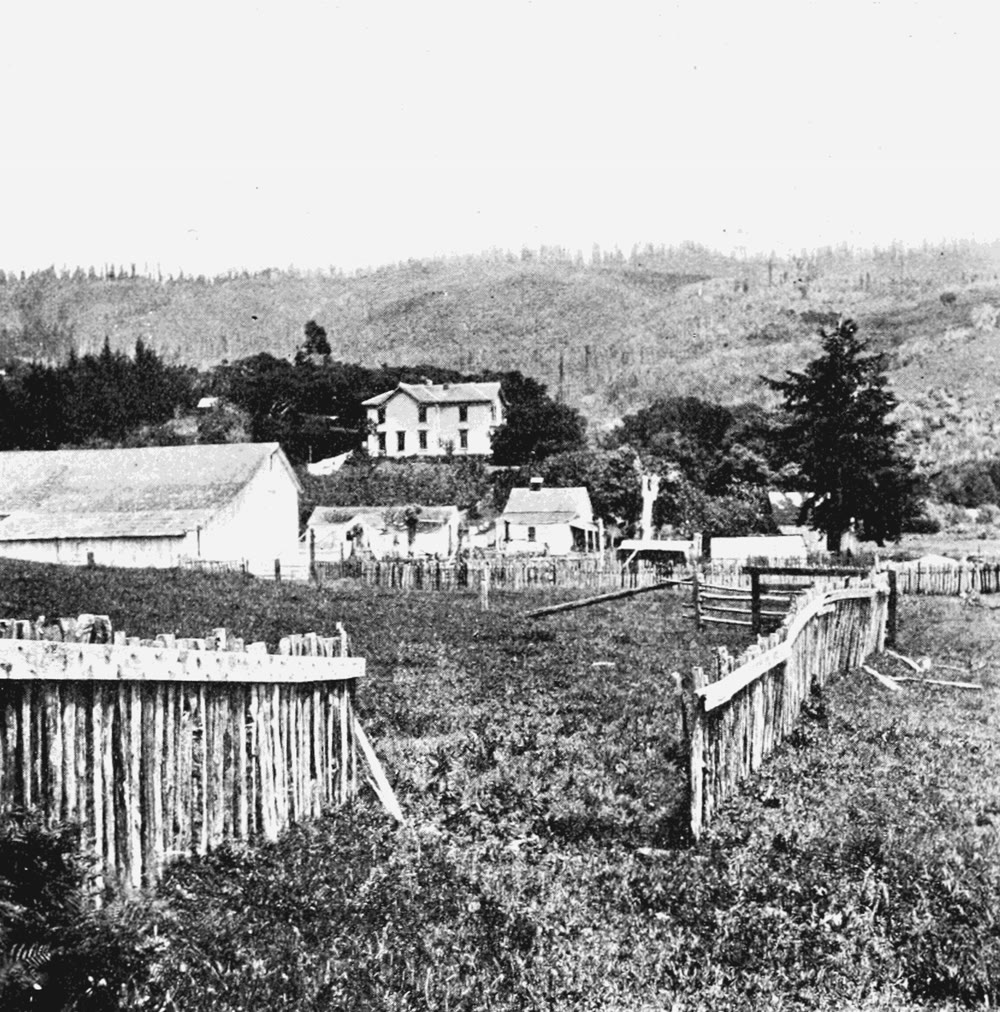
\includegraphics[height=5.6cm]{images/book3/b1-fence-1906.jpg}\hfill
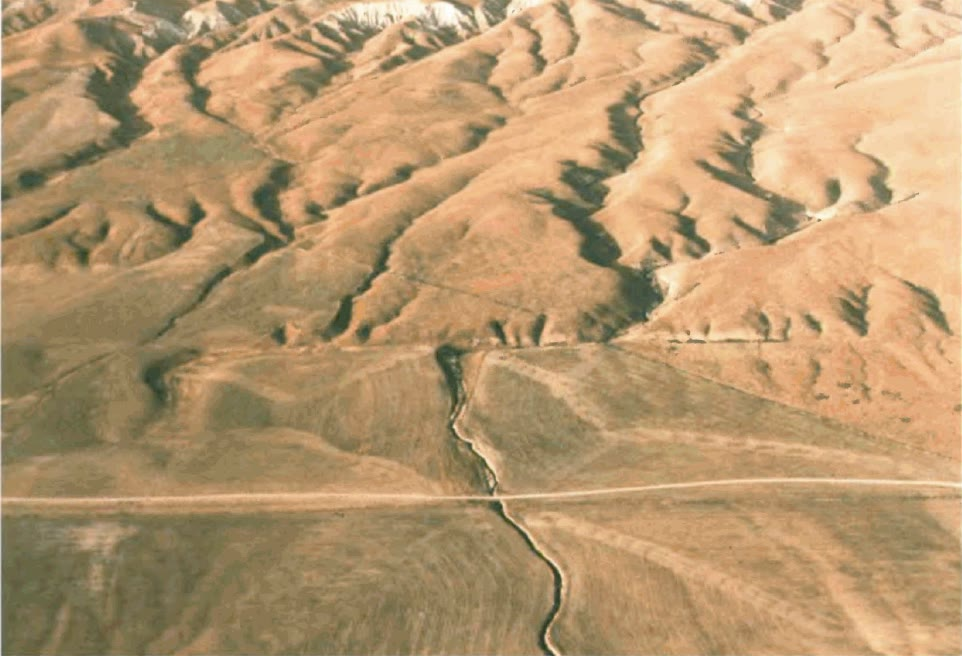
\includegraphics[height=5.6cm]{images/book3/b1-wallace-creek.jpg}
\par\smallskip{\small À esquerda: cercas em terras agrícolas do condado de Marin, ao norte de São Francisco, cortadas pela ruptura de 1906, publicadas no mesmo ano como ``terra separada pela falha do terremoto''. Fotografia de \emph{Popular Science Monthly}, vol.~69 (1906), domínio público. À direita: Wallace Creek, Carrizo Plain, vista do ar: o riacho desce das colinas (no alto), e onde cruza a falha de San Andreas, ao pé das colinas, seu canal se desloca lateralmente em \qty{130}{m}, o deslocamento acumulado ao longo de milhares de anos de terremotos. Fotografia:
R.~E.~Wallace, U.S. Geological Survey, domínio público. Ambas do Wikimedia Commons.}
\label{fig:b1:earthquake-source:offsets}
\end{omfigure}
% ledger: commons:psm-fence, commons:wallace-creek

A proposição dá uma média, não um calendário. Perto de Parkfield, na mesma falha, um terremoto de magnitude cerca de 6 em 1857 foi seguido por cinco outros, muito parecidos, no mesmo trecho de cerca de \qty{30}{km}, em intervalos de quase 22 anos até 1966; o próximo era esperado antes de 1993, e veio em 2004, com \omterm{def:b1:earthquake-source:mw}{magnitude de momento} 6.0 e sem qualquer sinal claro de alerta. A resistência de uma falha, o deslizamento de cada terremoto e o carregamento por seus vizinhos variam de um ciclo para o seguinte, e o \omterm{def:b1:earthquake-source:seismic-cycle}{ciclo sísmico} é mais bem descrito por um intervalo médio de recorrência e uma dispersão em torno dele do que por um período.
% ledger: pp1515:parkfield, bl85:parkfield, usgs:hist-mw, bakun:2005

Alguns segmentos de falha não se travam de modo nenhum. Entre Parkfield e San Juan Bautista, a seção central da falha de San Andreas rasteja: o deslizamento constante na falha absorve quase todo o movimento das placas, e pouca ou nenhuma deformação se acumula de cada lado, de modo que essa seção não tem grandes terremotos; a grande ruptura de 1857 começou em seu extremo sul, e a de 1906 parou em seu extremo norte. Uma falha que rasteja sobre parte de sua área está travada apenas em parte, o que é o coeficiente $c$ da proposição.
% ledger: pp1515:creep, pp1515:1906

\begin{inthefield}[Lendo terremotos passados em uma trincheira]
Os instrumentos registram terremotos há pouco mais de um século, bem menos que um ciclo da maioria das falhas. Paleossismólogos estendem o registro lendo o solo. Uma trincheira de alguns metros de profundidade é escavada através de uma falha ativa onde camadas de sedimento foram depositadas continuamente, em um pântano, em um lago ou em um pequeno leque aluvial. Em suas paredes, cada terremoto aparece como camadas cortadas e deslocadas pela falha e cobertas, sem ruptura, por camadas mais jovens; como uma escarpa enterrada por depósitos posteriores; como areia que se liquefez e subiu por fendas para se espalhar sobre a superfície da época. Turfa ou restos vegetais nas camadas logo abaixo e logo acima de cada ruptura são datados por radiocarbono, e assim delimitam a data de cada terremoto: um pântano na falha de San Andreas guarda o registro de doze.
Ao longo das costas, \omterm{def:b1:layered-earth:layers}{mantos} de areia depositados por tsunamis e pântanos que afundaram de repente, em cerca de um metro, soterrados sob lama de maré, registram os grandes terremotos de subducção. Na falha de San Andreas, a maior parte do deslizamento dos tempos históricos veio com terremotos de magnitude 6 ou mais.
\end{inthefield}
% ledger: pp1515:pallett, atwater:1987

\begin{history}[Harry Fielding Reid e a recuperação elástica]
Harry Fielding Reid, físico norte-americano, era membro da comissão estadual que estudou o terremoto de 1906. Ao comparar as posições de pontos medidos em 1851--1865, em 1874--1892 e depois do terremoto, ele constatou que pontos distantes nos dois lados da falha de San Andreas tinham se deslocado em cerca de \qty{3.2}{m} um em relação ao outro desde o primeiro levantamento, um pouco mais da metade do deslizamento de cerca de \qty{6}{m} na falha: meio século antes do terremoto, a deformação que rompeu a falha já estava pela metade acumulada. Somente forças elásticas poderiam ter movido o solo de forma tão súbita, e ele chamou o retorno súbito de \omterm{def:b1:earthquake-source:seismic-cycle}{recuperação elástica}. Publicou-a no segundo volume do relatório da comissão, em 1910; ainda é o principal modelo do \omterm{def:b1:earthquake-source:seismic-cycle}{ciclo sísmico}. O posicionamento por satélite desde então mediu a curvatura que ele só pôde inferir.
\end{history}
% ledger: reid:1910, pp1515:1906

\section{Momento sísmico e magnitude}\label{sec:b1:earthquake-source:moment}

O tamanho de um terremoto é a quantidade de deslizamento que ele produziu, sobre a área da falha que deslizou, ponderada pela rigidez das rochas.

\begin{definition}[Momento sísmico]\label{def:b1:earthquake-source:moment}
Seja um terremoto que desliza de uma quantidade média $D$ sobre uma ruptura de área $A$, em rochas de módulo de cisalhamento $\mu$ (a letra também nomeia um coeficiente de atrito, em \cref{ch:b1:stress-strain-rheology}; o contexto mostra qual). Seu \emph{momento sísmico}\index{momento sísmico} é
\[
  M_0 = \mu A D ,
\]
em newton metros.
\end{definition}
% ledger: usgs:gloss-moment

A unidade é a de um torque. Um deslizamento em uma falha emite as mesmas ondas que dois pares de forças opostas, dois binários, aplicados no foco, e o \omterm{def:b1:earthquake-source:moment}{momento sísmico} é o momento de cada binário (essa equivalência, o duplo binário, é demonstrada no Livro 5). O momento tem a dimensão de uma energia, mas não é uma: a energia irradiada como ondas é uma pequena fração dele. Para as rochas da \omterm{def:b1:layered-earth:layers}{crosta}, $\mu$ é tomado como \qty{30}{GPa}.
% ledger: kanamori:1977, sk:mu-locking

O momento é calculado hoje a partir das ondas de longo período registradas em todo o mundo. Para o terremoto de Tohoku, de 11 de março de 2011, a solução preferida do Serviço Geológico dos Estados Unidos dá $M_0 = \qty{5.59e22}{N.m}$. A falha deslizou sobre uma área de cerca de \qty{400}{km} de comprimento e \qty{150}{km} de largura; a definição então dá o deslizamento médio
\[
  D = \frac{M_0}{\mu A}
    = \frac{\num{5.59e22}}{\num{3e10}\times\num{4e5}\times\num{1.5e5}}
    \approx \qty{31}{m} ,
\]
e modelos da ruptura encontram até \qtyrange{50}{60}{m} em sua parte mais deslocada.
% ledger: usgs:tohoku-mt, usgs:tohoku-summary

A magnitude do Livro 1 foi calculada a partir da amplitude das ondas em um sismograma. Tais magnitudes medem as ondas de um período; quando uma ruptura é muito mais longa que o comprimento de onda delas, de poucos a cerca de cinquenta quilômetros, a amplitude deixa de crescer com seu tamanho, e a magnitude satura. A magnitude das ondas de corpo satura perto de 6.5, a das ondas de superfície perto de 8.3. Em 2011, o primeiro alerta de tsunami para Tohoku baseou-se em uma magnitude desse tipo, que fica aquém para terremotos de magnitude 8 ou mais, e subestimou as ondas. O momento não satura, e a magnitude é agora definida a partir dele.
% ledger: kanamori:1977, usgs:magtypes, jma:warning

\begin{definition}[Magnitude de momento]\label{def:b1:earthquake-source:mw}
A \emph{magnitude de momento}\index{magnitude de momento} de um terremoto de \omterm{def:b1:earthquake-source:moment}{momento sísmico} $M_0$, em newton metros, é
\[
  M_w = \tfrac23\left(\log_{10} M_0 - 9.1\right) .
\]
\end{definition}
% ledger: usgs:magtypes

Thomas Hanks e Hiroo Kanamori definiram a escala em 1979, com a constante 9.05 no lugar de 9.1, uma diferença de 0.03 em $M_w$; as constantes foram escolhidas para coincidir com as magnitudes antigas onde estas não saturam. A magnitude do Livro 1 é, para grandes terremotos, este número: para Tohoku,
$M_w = \tfrac23(\log_{10}\num{5.59e22} - 9.1) = \tfrac23(22.75 - 9.1) = 9.1$;
o grande terremoto chileno de 1960 e o terremoto do Alasca de 1964 têm \omterm{def:b1:earthquake-source:mw}{magnitudes de momento} de 9.5 e 9.2, tamanhos que as magnitudes antigas não podiam mostrar.
% ledger: hk:1979, kanamori:1977, usgs:hist-mw, usgs:tohoku-mt

\begin{proposition}[Uma unidade de magnitude]\label{prop:b1:earthquake-source:moment-steps}
O \omterm{def:b1:earthquake-source:moment}{momento sísmico} é $M_0 = 10^{1.5 M_w + 9.1}$ newton metros. Uma unidade de \omterm{def:b1:earthquake-source:mw}{magnitude de momento} o multiplica por $10^{1.5} \approx 31.6$, duas unidades por
$1000$. Se a energia irradiada for uma fração fixa do momento, ela cresce na mesma razão.
\end{proposition}

\begin{proof}
Resolvendo a definição para $M_0$ dá $\log_{10} M_0 = 1.5 M_w + 9.1$, e para dois terremotos
\[
  \log_{10}\frac{M_0'}{M_0} = 1.5\,(M_w' - M_w) ,
\]
que é $1.5$ para uma unidade e $3$ para duas. Se a energia irradiada é $E_s = k M_0$ com o mesmo $k$ para ambos, $E_s'/E_s = M_0'/M_0$.
\end{proof}

A aproximação de Kanamori, $E_s \approx M_0/(2\times10^4)$ (admitida), é a hipótese da última frase; o fator de cerca de 32 em energia por unidade de magnitude, encontrado no Livro 1, é esta proposição. Como $M_0 = \mu A D$ e o deslizamento de um terremoto cresce com o tamanho de sua ruptura, uma grande magnitude precisa de uma grande falha. A ruptura de 1906, com cerca de \qty{430}{km} de comprimento, rompeu a \omterm{def:b1:stress-strain-rheology:strength-envelope}{camada sismogênica} até cerca de \qty{15}{km} com um deslizamento médio de alguns metros:
com $D = \qty{4}{m}$, $M_0 = \num{3e10}\times\num{4.3e5}\times\num{1.5e4}
\times 4 = \qty{7.7e20}{N.m}$ e $M_w = 7.9$, a magnitude do catálogo.
Uma magnitude 9 precisa de uma ruptura de centenas de quilômetros de comprimento e mais de cem de largura, o que só as interfaces de \omterm{def:b1:geological-maps:attitude}{mergulho} suave das zonas de subducção oferecem.
% ledger: kanamori:1977, pp1515:1906, usgs:hist-mw, usgs:pp1515-thatcher

\section{Mecanismos focais}\label{sec:b1:earthquake-source:focal}

A onda P é a primeira a chegar a um sismômetro. Seu \omterm{def:b1:earthquake-source:focal-mechanism}{primeiro movimento}, o primeiro balanço do registro vertical, é para cima onde a onda chega como um empurrão, o solo comprimido e lançado para longe da fonte, e para baixo onde ela chega como um puxão. Em torno de um terremoto, empurrões e puxões se dispõem em um padrão que dá a orientação da falha e a \omterm{def:b1:geological-maps:attitude}{direção} do deslizamento.

\begin{proposition}[O sinal do primeiro movimento]\label{prop:b1:earthquake-source:first-motion}
Seja uma falha de normal ascendente $\mathbf n$ que desliza pelo vetor unitário $\mathbf d$
(o deslizamento do \omterm{def:b1:faults-folds-fabrics:fault-elements}{bloco superior} em relação ao inferior). A onda P que sai do foco na \omterm{def:b1:geological-maps:attitude}{direção} unitária $\mathbf x$ chega como empurrão se
$(\mathbf n\cdot\mathbf x)(\mathbf d\cdot\mathbf x) > 0$ e como puxão se
$(\mathbf n\cdot\mathbf x)(\mathbf d\cdot\mathbf x) < 0$. Os empurrões e os puxões preenchem assim quatro quadrantes, separados pelo plano da falha
($\mathbf n\cdot\mathbf x = 0$) e pelo plano perpendicular ao deslizamento ($\mathbf d\cdot\mathbf x = 0$).
\end{proposition}

\begin{proof}
Uma \omterm{def:b1:geological-maps:attitude}{direção} com $\mathbf n\cdot\mathbf x > 0$ aponta para o \omterm{def:b1:faults-folds-fabrics:fault-elements}{bloco superior}, que se move de $\mathbf d$ em relação ao inferior: a rocha à frente dele, onde $\mathbf d\cdot\mathbf x > 0$, é comprimida, e a rocha atrás dele, onde $\mathbf d\cdot\mathbf x < 0$, é puxada. Uma \omterm{def:b1:geological-maps:attitude}{direção} com
$\mathbf n\cdot\mathbf x < 0$ aponta para o \omterm{def:b1:faults-folds-fabrics:fault-elements}{bloco inferior}, que se move de $-\mathbf d$ em relação ao superior, de modo que os sinais se invertem. Em cada
caso o \omterm{def:b1:earthquake-source:focal-mechanism}{primeiro movimento} tem o sinal de $(\mathbf n\cdot\mathbf x)(\mathbf
d\cdot\mathbf x)$.
\end{proof}

O argumento dá apenas o sinal. A amplitude do \omterm{def:b1:earthquake-source:focal-mechanism}{primeiro movimento}, proporcional a $2(\mathbf n\cdot\mathbf x)(\mathbf d\cdot\mathbf x)$ e assim máxima a \ang{45} de ambos os planos e nula sobre eles, é admitida aqui (volume do Livro 5).

\begin{omfigure}
\begin{tikzpicture}[>={Stealth[length=5pt]}, font=\small, scale=0.95]
% map view around a vertical dextral fault striking north, the focus at the origin, rays leaving
% horizontally: pushes where (n.x)(d.x) > 0, i.e. in the NW and SE quadrants (beachballs.py,
% first_motion(0, 90, 180, x)). Stations at 20 azimuths on a circle of radius 2.3.
\fill[omThm!22] (0,0) -- (0,2.8) arc[start angle=90, end angle=180, radius=2.8] -- cycle;
\fill[omThm!22] (0,0) -- (0,-2.8) arc[start angle=270, end angle=360, radius=2.8] -- cycle;
\draw[black!40, line width=0.4pt] (0,0) circle[radius=2.8];
\draw[fault, line width=1.3pt] (0,-3.1) -- (0,3.1) node[above, font=\scriptsize] {falha (plano nodal)};
\draw[black, dashed, line width=0.7pt] (-3.1,0) -- (3.1,0) node[right, font=\scriptsize, align=left] {plano\\ auxiliar};
% slip: the west block moves north, the east block south
\draw[->, line width=1pt] (-0.3,-0.8) -- (-0.3,0.8);
\draw[->, line width=1pt] (0.3,0.8) -- (0.3,-0.8);
% stations
\foreach \a in {9,27,...,351} {
  \pgfmathsetmacro{\fm}{-sin(\a)*cos(\a)}  % (n.x)(d.x) with n = east, d = south, x = (sin a, cos a)
  \pgfmathparse{\fm>0 ? 1 : 0}
  \ifnum\pgfmathresult=1
    \fill[black] ({2.3*sin(\a)},{2.3*cos(\a)}) circle[radius=0.11];
  \else
    \draw[black, fill=white, line width=0.6pt] ({2.3*sin(\a)},{2.3*cos(\a)}) circle[radius=0.11];
  \fi
}
% P and T axes
\draw[<-, omProp, line width=1.1pt] ({0.7*sin(45)},{0.7*cos(45)}) -- ({1.6*sin(45)},{1.6*cos(45)}) node[above right, font=\scriptsize, inner sep=1pt] {P};
\draw[<-, omProp, line width=1.1pt] ({0.7*sin(225)},{0.7*cos(225)}) -- ({1.6*sin(225)},{1.6*cos(225)});
\draw[->, omProp, line width=1.1pt] ({0.7*sin(315)},{0.7*cos(315)}) -- ({1.6*sin(315)},{1.6*cos(315)}) node[above left, font=\scriptsize, inner sep=1pt] {T};
\draw[->, omProp, line width=1.1pt] ({0.7*sin(135)},{0.7*cos(135)}) -- ({1.6*sin(135)},{1.6*cos(135)});
\fill (0,0) circle[radius=0.06];
% legend
\begin{scope}[xshift=4.6cm, yshift=2.4cm]
  \fill[black] (0,0) circle[radius=0.11]; \node[anchor=west, font=\scriptsize] at (0.2,0) {empurrão: primeiro movimento para cima};
  \draw[black, fill=white, line width=0.6pt] (0,-0.5) circle[radius=0.11]; \node[anchor=west, font=\scriptsize] at (0.2,-0.5) {puxão: primeiro movimento para baixo};
  \fill[omThm!22] (-0.12,-1.12) rectangle (0.12,-0.88); \node[anchor=west, font=\scriptsize] at (0.2,-1.0) {quadrante compressional};
  \draw[->] (-0.1,-1.6) -- (-0.1,-1.25); \node[anchor=west, font=\scriptsize] at (0.2,-1.42) {N};
\end{scope}
\end{tikzpicture}
\par\smallskip{\small \omterm{def:b1:earthquake-source:focal-mechanism}{Primeiros movimentos} em torno de uma falha \omterm{def:b1:faults-folds-fabrics:fault-types}{dextral} vertical de \omterm{def:b1:geological-maps:attitude}{direção} norte, vista de cima, para ondas que saem do foco horizontalmente em direção a estações em todo o seu redor. Setas pretas: o deslizamento dos dois blocos. Os empurrões preenchem os quadrantes noroeste e sudeste, os puxões os outros dois; a falha e o \omterm{def:b1:earthquake-source:focal-mechanism}{plano auxiliar} os separam. O \omterm{def:b1:earthquake-source:focal-mechanism}{eixo P} (setas apontando para dentro) divide ao meio os quadrantes de puxão, o \omterm{def:b1:earthquake-source:focal-mechanism}{eixo T} (setas apontando para fora) os quadrantes de empurrão. Um deslizamento \omterm{def:b1:faults-folds-fabrics:fault-types}{sinistral} no plano tracejado, com o bloco ao sul dele se movendo para leste, daria exatamente o mesmo padrão
(\cref{prop:b1:earthquake-source:auxiliary}).}
\label{fig:b1:earthquake-source:quadrants}
\end{omfigure}

O produto $(\mathbf n\cdot\mathbf x)(\mathbf d\cdot\mathbf x)$ não muda quando $\mathbf n$ e $\mathbf d$ são trocados. Essa simetria é o fato central dos mecanismos focais.

\begin{definition}[Mecanismo focal, plano nodal, plano auxiliar, eixo P, eixo T]\label{def:b1:earthquake-source:focal-mechanism}
O \emph{primeiro movimento}\index{primeiro movimento} de uma onda P em um sismômetro é a \omterm{def:b1:geological-maps:attitude}{direção}, para cima ou para baixo, do primeiro movimento do solo no registro vertical. O \emph{mecanismo focal}\index{mecanismo focal} de um terremoto é a orientação do plano da falha e a \omterm{def:b1:geological-maps:attitude}{direção} do deslizamento sobre ele, como encontrados a partir de suas ondas sísmicas. Os dois planos perpendiculares através do foco que separam os empurrões dos puxões são seus \emph{planos nodais}\index{plano nodal}; um é o plano da falha, e o outro, perpendicular ao deslizamento, é o \emph{plano auxiliar}\index{plano auxiliar}. O \emph{eixo P}\index{eixo P} e o \emph{eixo T}\index{eixo T} são as direções a \ang{45} de ambos os planos nodais, no meio dos quadrantes de puxão e de empurrão:
\[
  \mathbf P = \frac{\mathbf n - \mathbf d}{\sqrt2}, \qquad
  \mathbf T = \frac{\mathbf n + \mathbf d}{\sqrt2} .
\]
\end{definition}
% ledger: yvo:beachball, usgs:gloss-moment

\begin{proposition}[Os dois planos nodais]\label{prop:b1:earthquake-source:auxiliary}
Um deslizamento $\mathbf d$ sobre o plano de normal $\mathbf n$ e um deslizamento $\mathbf n$ sobre o plano de normal $\mathbf d$ dão os mesmos \omterm{def:b1:earthquake-source:focal-mechanism}{primeiros movimentos} em toda \omterm{def:b1:geological-maps:attitude}{direção}. Os \omterm{def:b1:earthquake-source:focal-mechanism}{primeiros movimentos} determinam, portanto, os dois \omterm{def:b1:earthquake-source:focal-mechanism}{planos nodais}, os \omterm{def:b1:earthquake-source:focal-mechanism}{eixos P} e T e o sentido do deslizamento sobre cada plano, mas não dizem qual \omterm{def:b1:earthquake-source:focal-mechanism}{plano nodal} é a falha.
\end{proposition}

\begin{proof}
O sinal de $(\mathbf n\cdot\mathbf x)(\mathbf d\cdot\mathbf x)$ não muda pela troca de $\mathbf n$ e $\mathbf d$; os planos $\mathbf n\cdot\mathbf x = 0$ e $\mathbf d\cdot\mathbf x = 0$ são trocados, e $\mathbf n \pm \mathbf d$ não mudam. Um par $(\mathbf n, \mathbf d)$ e o par $(-\mathbf n, -\mathbf d)$, que descreve o mesmo deslizamento visto do outro bloco, também dão o mesmo produto. Nada nos \omterm{def:b1:earthquake-source:focal-mechanism}{primeiros movimentos} distingue as duas descrições.
\end{proof}

Para decidir qual \omterm{def:b1:earthquake-source:focal-mechanism}{plano nodal} deslizou, os sismólogos usam outras evidências: o plano ao longo do qual se alinham as réplicas, a falha vista na superfície, o limite de placas em que o terremoto está. Para o grande terremoto de Sumatra--Andamão de 2004, os dois \omterm{def:b1:earthquake-source:focal-mechanism}{planos nodais} mergulham \ang{8} para nordeste e \ang{83} para sudoeste. Os terremotos anteriores da região e os modelos de placas situam a laje afundante ao longo de um plano que mergulha suavemente para nordeste, e o plano raso é tomado como a falha: o terremoto rompeu a interface de placas da zona de subducção, e suas réplicas se espalharam por mais de \qty{1300}{km}.
% ledger: usgs:sumatra-mt, usgs:sumatra-summary

Como o \omterm{def:b1:earthquake-source:focal-mechanism}{eixo P} jaz no meio dos puxões e o \omterm{def:b1:earthquake-source:focal-mechanism}{eixo T} no meio dos empurrões, eles são muitas vezes lidos como as direções das tensões compressivas máxima e mínima, $\sigma_1$ e $\sigma_3$. São apenas aproximações delas. Uma falha nova se forma a $\ang{45} - \phi/2$ de $\sigma_1$, não a \ang{45} (\cref{ch:b1:stress-strain-rheology}), e uma falha antiga pode deslizar a um ângulo ainda diferente, de modo que os eixos de um só terremoto podem estar a dezenas de graus das \omterm{def:b1:stress-strain-rheology:principal}{tensões principais}; as tensões de uma região são encontradas a partir dos mecanismos de muitos terremotos juntos.

Um \omterm{def:b1:earthquake-source:focal-mechanism}{mecanismo focal} vive sobre uma esfera em torno do foco. Ele é desenhado na metade inferior dessa esfera, que todo raio para uma estação distante atravessa, projetada sobre um disco: um raio de vetor unitário $\mathbf x = (E, N, U)$, com $U \le 0$, é marcado em
\[
  (X, Y) = \frac{(E, N)}{\sqrt{1 - U}} ,
\]
a vertical no centro e a horizontal no círculo unitário. Esta
projeção preserva áreas (admitida; as projeções da esfera são estudadas no
volume do terceiro ano), de modo que cada quadrante cobre sua parcela verdadeira do disco. Os
quadrantes de compressão são sombreados; a figura se chama bola de praia.
% ledger: yvo:beachball

\begin{omfigure}
\begin{tikzpicture}[font=\small]
% lower-hemisphere equal-area beach balls, compressional quadrants shaded (figdata/bachelor-1/beachballs.py)
\foreach \n/\c/\t/\x in {normal/2/{(a) falha normal\\ $090/60$, rake \ang{-90}}/0,
                         reverse/1/{(b) falha inversa\\ $090/30$, rake \ang{90}}/3.65,
                         strikeslip/2/{(c) falha transcorrente\\ $090/90$, rake \ang{180}}/7.3,
                         tohoku/2/{(d) Tohoku, 2011\\ $282/8$, rake \ang{78}}/10.95} {
  \begin{axis}[at={(\x cm,0)}, anchor=center, width=2.9cm, height=2.9cm, scale only axis,
      axis equal image, xmin=-1.04, xmax=1.04, ymin=-1.04, ymax=1.04, hide axis, clip=false]
    \fill[white] (axis cs:0,0) circle[radius=1];
    \addplot[fill=omThm!55, draw=none] table[x=X, y=Y] {figdata/out/bachelor-1-beachballs-\n-c1.dat};
    \ifnum\c=2
      \addplot[fill=omThm!55, draw=none] table[x=X, y=Y] {figdata/out/bachelor-1-beachballs-\n-c2.dat};
    \fi
    \addplot[black, line width=0.6pt] table[x=X, y=Y] {figdata/out/bachelor-1-beachballs-\n-p1.dat};
    \addplot[black, line width=0.6pt] table[x=X, y=Y] {figdata/out/bachelor-1-beachballs-\n-p2.dat};
    \draw[black, line width=0.8pt] (axis cs:0,0) circle[radius=1];
    \draw[black, line width=0.5pt] (axis cs:0,1) -- (axis cs:0,1.12) node[above, font=\scriptsize, inner sep=1pt] {N};
    \addplot[only marks, mark=none, nodes near coords={\textbf{P}}, nodes near coords align=center, every node near coord/.append style={font=\scriptsize, inner sep=0pt}] table[x=X, y=Y] {figdata/out/bachelor-1-beachballs-\n-P.dat};
    \addplot[only marks, mark=none, nodes near coords={\textbf{T}}, nodes near coords align=center, every node near coord/.append style={font=\scriptsize, inner sep=0pt}] table[x=X, y=Y] {figdata/out/bachelor-1-beachballs-\n-T.dat};
    \node[anchor=north, align=center, font=\scriptsize] at (axis cs:0,-1.12) {\t};
  \end{axis}
}
\end{tikzpicture}
\par\smallskip{\small Bolas de praia: o hemisfério inferior em torno do foco, em projeção de áreas iguais, norte para cima, os quadrantes de empurrão sombreados, P e T marcando os eixos (uma letra é deslocada para dentro quando seu eixo está perto da borda). Cada mecanismo é dado pela \omterm{def:b1:geological-maps:attitude}{atitude} de um \omterm{def:b1:earthquake-source:focal-mechanism}{plano nodal}, sentido e \omterm{def:b1:geological-maps:attitude}{mergulho}, e pelo \omterm{def:b1:faults-folds-fabrics:fault-elements}{rake} do deslizamento sobre ele. (a) Uma \omterm{def:b1:faults-folds-fabrics:fault-types}{falha normal} mergulhando \ang{60} para leste: o quadrante de puxão ocupa o centro. (b) Uma \omterm{def:b1:faults-folds-fabrics:fault-types}{falha inversa} mergulhando \ang{30} para leste: o quadrante de empurrão ocupa o centro. (c) Uma \omterm{def:b1:faults-folds-fabrics:fault-types}{falha transcorrente} vertical: quatro quadrantes se encontram no centro. (d) O terremoto de Tohoku de 2011 (tensor de momento do Serviço Geológico dos Estados Unidos): um empurrão em um plano que mergulha \ang{8} em direção a $282$, sob o Japão, com o \omterm{def:b1:earthquake-source:focal-mechanism}{plano auxiliar} íngreme a leste.}
\label{fig:b1:earthquake-source:beachballs}
\end{omfigure}
% ledger: usgs:tohoku-mt

Os sismólogos dão um mecanismo pela \omterm{def:b1:geological-maps:attitude}{direção}, \omterm{def:b1:geological-maps:attitude}{mergulho} e \omterm{def:b1:faults-folds-fabrics:fault-elements}{rake} de cada \omterm{def:b1:earthquake-source:focal-mechanism}{plano nodal}; a \omterm{def:b1:geological-maps:attitude}{direção} é o \omterm{def:b1:geological-maps:attitude}{sentido de mergulho} menos \ang{90}, como em
\cref{ch:b1:faults-folds-fabrics}. Para Tohoku, os planos são
$192/8/78$ e $24/81/91$ em direção, \omterm{def:b1:geological-maps:attitude}{mergulho} e \omterm{def:b1:faults-folds-fabrics:fault-elements}{rake}, e os \omterm{def:b1:earthquake-source:focal-mechanism}{eixos P} e T têm \omterm{def:b1:field-lab-methods-1:trend-plunge}{rumo}
$113$ e $296$ e \omterm{def:b1:field-lab-methods-1:trend-plunge}{caimento} \ang{36} e \ang{53}.
O \omterm{def:b1:earthquake-source:focal-mechanism}{plano auxiliar} segue do plano da falha: sua normal é $\mathbf d$ e seu deslizamento é $\mathbf n$, de modo que se encontra calculando $\mathbf n$ e $\mathbf d$ a partir da \omterm{def:b1:geological-maps:attitude}{direção}, do \omterm{def:b1:geological-maps:attitude}{mergulho} e do \omterm{def:b1:faults-folds-fabrics:fault-elements}{rake}, trocando-os, e lendo de volta a \omterm{def:b1:geological-maps:attitude}{direção}, o \omterm{def:b1:geological-maps:attitude}{mergulho} e o \omterm{def:b1:faults-folds-fabrics:fault-elements}{rake} (exercício~\ref{exo:b1:earthquake-source:7}).
% ledger: usgs:tohoku-mt

\begin{method}[Lendo uma bola de praia]\label{met:b1:earthquake-source:beachball}
\begin{enumerate}
  \item Olhe para o centro, que é a vertical. Sombreado (um empurrão direto para baixo): uma componente inversa ou de empurrão; branco: uma componente normal. Dois diâmetros retos que se cruzam no centro: um mecanismo transcorrente.
  \item Encontre os dois \omterm{def:b1:earthquake-source:focal-mechanism}{planos nodais}, as curvas que delimitam os quadrantes. Um plano que passa pelo centro é vertical; um plano mergulha para o lado do centro em que sua curva se encontra, tanto mais suavemente quanto mais perto da borda estiver a curva.
  \item Encontre o \omterm{def:b1:earthquake-source:focal-mechanism}{eixo T} no meio dos quadrantes sombreados e o \omterm{def:b1:earthquake-source:focal-mechanism}{eixo P} no meio dos brancos: o solo foi encurtado ao longo de P e alongado ao longo de T.
  \item Para cada \omterm{def:b1:earthquake-source:focal-mechanism}{plano nodal}, leia ou calcule o \omterm{def:b1:faults-folds-fabrics:fault-elements}{rake}, e dê nome à falha que ele seria com \cref{def:b1:faults-folds-fabrics:fault-types}. Os dois planos sempre compartilham o sentido de deslizamento de \omterm{def:b1:geological-maps:attitude}{mergulho}, normal ou inverso, e têm sentidos transcorrentes opostos: um mecanismo transcorrente dá um plano \omterm{def:b1:faults-folds-fabrics:fault-types}{dextral} e um \omterm{def:b1:faults-folds-fabrics:fault-types}{sinistral}.
  \item Escolha o plano da falha pelas réplicas, pela geologia ou pelo limite de placas.
\end{enumerate}
\end{method}

\begin{inthelab}[No observatório sismológico]
\begin{minipage}[t]{0.6\linewidth}\vspace{0pt}
Em minutos após um grande terremoto, suas ondas foram registradas por centenas de estações, e os dados chegam aos analistas dos observatórios quase em tempo real. As primeiras chegadas da onda P, que chegam às estações tanto mais tarde quanto mais distantes elas estão, são marcadas nos registros para localizar o foco. Em seguida, as ondas longas e lentas registradas nas dezenas de minutos seguintes são comparadas com ondas calculadas para fontes de teste; a fonte cujas ondas melhor se ajustam dá o tensor de momento, que contém em conjunto o \omterm{def:b1:earthquake-source:moment}{momento sísmico}, a \omterm{def:b1:earthquake-source:mw}{magnitude de momento} e os dois \omterm{def:b1:earthquake-source:focal-mechanism}{planos nodais}. Para terremotos pequenos, fracos demais para isso, os analistas leem os \omterm{def:b1:earthquake-source:focal-mechanism}{primeiros movimentos} nos registros mais próximos e ajustam os \omterm{def:b1:earthquake-source:focal-mechanism}{planos nodais} a eles, do modo descrito nesta seção.
Cada solução é publicada com suas incertezas, e revisada à medida que chegam mais dados.
\end{minipage}\hfill
\begin{minipage}[t]{0.36\linewidth}\vspace{0pt}
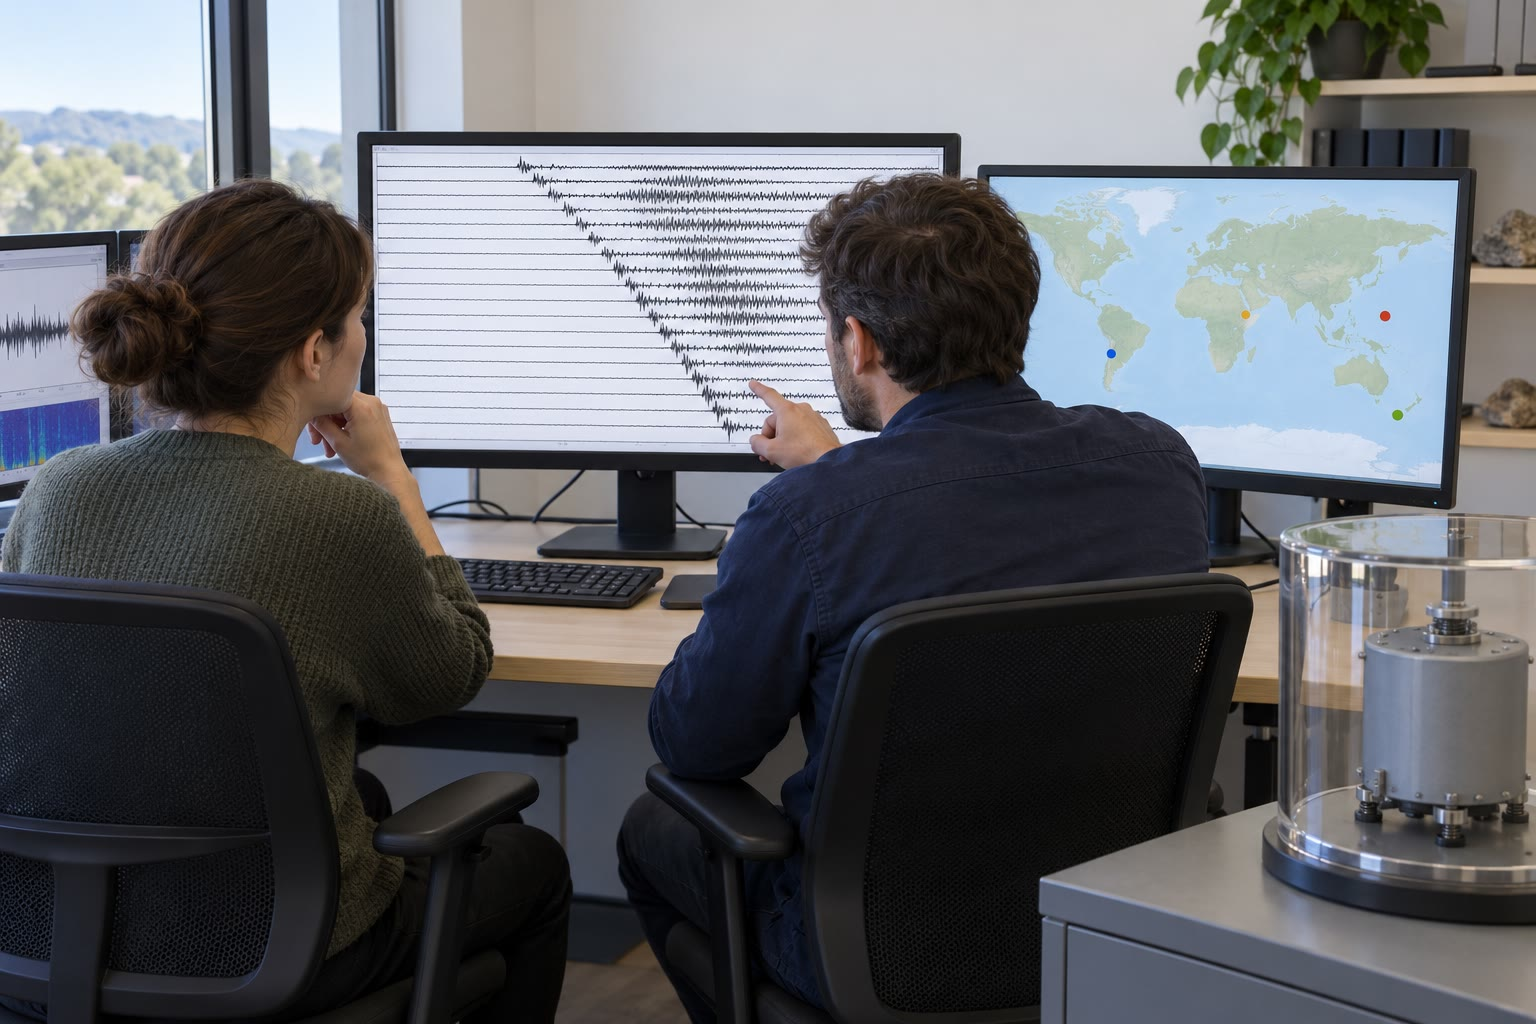
\includegraphics[width=\linewidth]{images/book3/ai/b1-seismic-analysis.jpg}

{\scriptsize Sismólogos lendo uma seção de registros, os traços de um
terremoto em estações ordenadas por distância (ilustração por IA).}
\end{minipage}
\end{inthelab}
% ledger: yvo:beachball

\section{Medindo o carregamento: geodésia}\label{sec:b1:earthquake-source:geodesy}

Entre os terremotos, uma falha travada é invisível aos sismômetros, mas o solo em torno dela se move. Estações permanentes de posicionamento por satélite medem esse movimento, e a maneira como suas velocidades mudam através de uma falha diz quão profundamente ela está travada.

\begin{definition}[Profundidade de travamento]\label{def:b1:earthquake-source:locking-depth}
A \emph{profundidade de travamento}\index{profundidade de travamento} de uma falha é a profundidade até a qual ela está travada entre os terremotos, abaixo da qual a falha desliza de modo constante à taxa de longo prazo; é a profundidade da parte da falha que desliza no próximo terremoto.
\end{definition}
% ledger: usgs:pp1515-thatcher

\begin{proposition}[Velocidade interssísmica através de uma falha transcorrente]\label{prop:b1:earthquake-source:interseismic}
Seja uma \omterm{def:b1:faults-folds-fabrics:fault-types}{falha transcorrente} vertical em um semiespaço elástico, travada da superfície até a profundidade $D$, e deslizando à taxa $V$ abaixo dela. A velocidade da superfície paralela à falha, à distância $x$ dela, é
\[
  v(x) = \frac{V}{\pi}\arctan\frac{x}{D} .
\]
Se a falha então desliza de $s$ da superfície até a profundidade $D$ em um terremoto, a superfície se move de $u(x) = (s/\pi)\arctan(D/x)$ para $x > 0$, e de
$-u(-x)$ para $x < 0$.
\end{proposition}
\admitted

Este modelo, devido a Savage e Burford, é a forma mais simples da \omterm{def:b1:earthquake-source:seismic-cycle}{recuperação elástica}, e a curva da cerca da primeira figura. Suas propriedades seguem da fórmula.

\begin{proposition}[Lendo o perfil interssísmico]\label{prop:b1:earthquake-source:profile}
No modelo de \cref{prop:b1:earthquake-source:interseismic}:
\begin{enumerate}[label=(\alph*)]
  \item longe da falha a velocidade tende a $\pm V/2$, as duas placas movendo-se a $V$ uma em relação à outra;
  \item metade da variação da velocidade através da falha ocorre a uma distância $D$ dela: $v(\pm D) = \pm V/4$;
  \item a taxa de \omterm{def:b1:stress-strain-rheology:strain}{deformação de cisalhamento} da superfície, $\mathrm dv/\mathrm dx$, é máxima sobre a falha, onde vale $V/(\pi D)$;
  \item se a falha, após carregar durante o tempo $t$, desliza de $s = Vt$ em um terremoto, o solo termina deslocado de $\pm s/2$ em toda parte de cada lado: o ciclo não deixa curvatura permanente, apenas o deslocamento $s$ sobre a falha.
\end{enumerate}
\end{proposition}

\begin{proof}
(a) $\arctan(x/D) \to \pm\pi/2$ quando $x \to \pm\infty$. (b) $\arctan 1 = \pi/4$, logo $v(D) = V/4$, e $v$ é ímpar. (c) $\mathrm dv/\mathrm dx = (V/\pi D)/(1 +
x^2/D^2)$, máximo em $x = 0$. (d) Para $x > 0$, o carregamento deslocou o solo de $t\,v(x) = (s/\pi)\arctan(x/D)$ e o terremoto de $(s/\pi)\arctan(D/x)$; como $\arctan y + \arctan(1/y) = \pi/2$ para $y > 0$, a soma é $s/2$. O mesmo vale com os sinais invertidos para $x < 0$.
\end{proof}

A propriedade (b) dá a \omterm{def:b1:earthquake-source:locking-depth}{profundidade de travamento} a partir de um perfil de estações: é a distância da falha em que a velocidade mudou de um quarto de $V$ em relação ao seu valor sobre a falha. Um travamento raso concentra a deformação perto da falha (figura abaixo), um travamento profundo a espalha por uma faixa larga. Ao longo do sistema de San Andreas, as \omterm{def:b1:earthquake-source:locking-depth}{profundidades de travamento} encontradas pela geodésia vão de quase 0, em segmentos que rastejam, a \qty{26}{km}, e concordam com as profundidades dos terremotos: a parte travada é a \omterm{def:b1:stress-strain-rheology:strength-envelope}{camada sismogênica} de
\cref{ch:b1:stress-strain-rheology}. Para uma taxa de deslizamento de
\qty{34}{mm.yr^{-1}} e uma \omterm{def:b1:earthquake-source:locking-depth}{profundidade de travamento} de \qty{15}{km}, a taxa de \omterm{def:b1:stress-strain-rheology:strain}{deformação de cisalhamento}
na falha é $\num{0.034}/(\pi\times\num{15000}) = \num{7.2e-7}$ por ano,
que curva uma linha através da falha em menos de um milímetro por quilômetro em um ano, mas armazena, ao longo de dois séculos, os vários metros de deslizamento de um grande terremoto.
% ledger: sk:mu-locking, usgs:pp1515-wallace, usgs:pp1515-thatcher

\begin{omfigure}
\begin{tikzpicture}[font=\small]
\begin{axis}[omrecord, width=11cm, height=5.6cm, xmin=-100, xmax=100, ymin=-19, ymax=19,
    xlabel={distância da falha $x$ (km)}, ylabel={velocidade $v$ (\unit{mm.yr^{-1}})},
    legend style={font=\scriptsize, at={(0.02,0.96)}, anchor=north west}, legend cell align=left]
  \addplot[omDef, line width=0.9pt, dashed] table[x=x, y=v5] {figdata/out/bachelor-1-interseismic-profiles.dat};
  \addplot[omThm, line width=1.1pt] table[x=x, y=v15] {figdata/out/bachelor-1-interseismic-profiles.dat};
  \addplot[omProp, line width=0.9pt, dotted] table[x=x, y=v25] {figdata/out/bachelor-1-interseismic-profiles.dat};
  \legend{$D = \qty{5}{km}$, $D = \qty{15}{km}$, $D = \qty{25}{km}$}
  \draw[black!50, dashed] (axis cs:-100,17) -- (axis cs:100,17);
  \draw[black!50, dashed] (axis cs:-100,-17) -- (axis cs:100,-17);
  \node[anchor=north west, font=\scriptsize] at (axis cs:-30,17) {$+V/2$};
  \node[anchor=south west, font=\scriptsize] at (axis cs:30,-17) {$-V/2$};
  \draw[black!60] (axis cs:0,-19) -- (axis cs:0,19);
  \node[anchor=east, font=\scriptsize] at (axis cs:-1,5) {falha};
\end{axis}
\end{tikzpicture}
\par\smallskip{\small Velocidade do solo paralela a uma \omterm{def:b1:faults-folds-fabrics:fault-types}{falha transcorrente} travada, em relação ao traço da falha, para uma taxa de deslizamento $V = \qty{34}{mm.yr^{-1}}$, a de San Andreas em Wallace Creek, e três \omterm{def:b1:earthquake-source:locking-depth}{profundidades de travamento} (\cref{prop:b1:earthquake-source:interseismic}). Quanto mais raso o travamento, mais estreita a faixa em que a velocidade muda.}
\label{fig:b1:earthquake-source:interseismic}
\end{omfigure}
% ledger: usgs:pp1515-wallace

Medidas por posicionamento por satélite registram o solo em poucos pontos. Satélites de radar o medem em toda parte: duas imagens de radar da mesma área, tomadas da mesma órbita em momentos diferentes, são comparadas onda por onda, e a diferença de fase mapeia a mudança da distância entre o solo e o satélite, ponto por ponto, a cada cem metros, sem uma rede de estações montada de antemão. O primeiro mapa desse tipo, de um grande terremoto californiano de 1992, mostrou seu deslocamento cossísmico em uma única imagem e concordou com o deslizamento medido no campo e por levantamento; a técnica, a interferometria de radar, pertence ao volume do Livro 5.
% ledger: massonnet:1993

\section{Com que frequência: a lei de Gutenberg--Richter}\label{sec:b1:earthquake-source:gr}

Terremotos pequenos são muito mais comuns que os grandes, e de modo notavelmente regular.

\begin{proposition}[Lei de Gutenberg--Richter]\label{prop:b1:earthquake-source:gutenberg-richter}
Em uma região e um período\index{lei de Gutenberg--Richter}, o número $N$ de terremotos de magnitude pelo menos
$M$ segue
\[
  \log_{10} N = a - bM ,
\]
para cada $M$ acima da \omterm{def:b1:earthquake-source:b-value}{magnitude de completude} do catálogo, com constantes $a$ e $b$ que dependem da região; $b$ é próximo de 1 na maioria das regiões ativas.
\end{proposition}
\admitted
% ledger: fd:1993, gr:1944

A lei é um resultado da observação, publicada por Beno Gutenberg e Charles Richter para a Califórnia em 1944 e desde então encontrada em toda parte; nenhuma teoria ainda a deriva, nem o valor de $b$.
% ledger: gr:1944

\begin{definition}[Valor b, magnitude de completude]\label{def:b1:earthquake-source:b-value}
A constante $b$ da \omterm{prop:b1:earthquake-source:gutenberg-richter}{lei de Gutenberg--Richter} de uma região é seu \emph{valor b}\index{valor b}. A \emph{magnitude de completude}\index{magnitude de completude} de um catálogo é a menor magnitude acima da qual ele registra todo terremoto da região e do período.
\end{definition}

Um \omterm{def:b1:earthquake-source:b-value}{valor b} de 1 significa dez vezes menos terremotos para cada unidade de magnitude. Abaixo da \omterm{def:b1:earthquake-source:b-value}{magnitude de completude}, as contagens ficam aquém da reta, pois terremotos pequenos são registrados por poucas estações para serem localizados: a lei parece curvar-se, e $b$ precisa ser medido acima dela. Para a Terra inteira, dividida em terremotos rasos, intermediários e profundos, os valores medidos ficam entre 0.72 e 1.34, mas diferem por \qty{30}{\percent} ou mais de um catálogo, faixa de magnitude ou método para outro: um valor distante de 1 é antes de tudo um motivo para verificar o catálogo.
% ledger: fd:1993

\begin{omfigure}
\begin{tikzpicture}[font=\small]
\begin{axis}[omrecord, width=6.4cm, height=5.8cm, ymode=log, xmin=5.8, xmax=9.3, ymin=0.01, ymax=300,
    xlabel={magnitude $M$}, ylabel={eventos de magnitude $\ge M$ por ano},
    log basis y=10, title={(a) frequência e magnitude}, title style={font=\small}]
  \addplot[omProp, line width=0.9pt, domain=5.8:9.3] table[x=M, y=rate] {figdata/out/bachelor-1-gutenberg_richter-fit.dat};
  \addplot[only marks, mark=*, mark size=1.3pt, omDef] table[x=M, y=rate] {figdata/out/bachelor-1-gutenberg_richter-counts.dat};
  \draw[black!50, dashed] (axis cs:7.5,0.01) -- (axis cs:7.5,300);
  \node[anchor=south west, font=\scriptsize, omProp] at (axis cs:8.45,0.5) {$b = 1.01$};
  \node[anchor=north west, font=\scriptsize, align=left] at (axis cs:7.55,200) {ajustado em\\ $6.0 \le M \le 7.5$};
\end{axis}
\begin{axis}[omrecord, at={(7.6cm,0)}, width=6.4cm, height=5.8cm, xmin=5.8, xmax=9.3, ymin=0, ymax=1.05,
    xlabel={magnitude $M$}, ylabel={fração do momento dos eventos $\ge M$},
    title={(b) para onde vai o momento}, title style={font=\small}]
  \addplot[const plot, omDef, line width=0.9pt] table[x=M, y=share] {figdata/out/bachelor-1-gutenberg_richter-moment.dat};
\end{axis}
\end{tikzpicture}
\par\smallskip{\small Os \num{7031} terremotos de magnitude 6 ou mais no mundo, 1976--2025 (catálogo do Serviço Geológico dos Estados Unidos). (a) O número anual de terremotos de magnitude ao menos $M$; a reta é o ajuste por mínimos quadrados de $\log_{10} N$ contra $M$ de 6.0 a 7.5, onde cada contagem excede 200:
$\log_{10} N = 8.20 - 1.01\,M$ por ano. Acima da magnitude 8 os poucos eventos ficam abaixo da reta. (b) A fração do \omterm{def:b1:earthquake-source:moment}{momento sísmico} total liberado pelos terremotos de magnitude ao menos $M$, cada momento calculado como
$10^{1.5M + 9.1}$\,\unit{N.m}: os 40 terremotos de magnitude 8 ou mais liberaram \qty{63}{\percent} dele.}
\label{fig:b1:earthquake-source:gutenberg-richter}
\end{omfigure}
% ledger: data:usgs-comcat (fit and shares computed in figdata/bachelor-1/gutenberg_richter.py)

Para o catálogo mundial da figura, a lei com $a = 8.20$ e $b = 1.01$ prevê 14 terremotos de magnitude 7 ou mais por ano, como observado, e 1.35 de magnitude 8 ou mais, enquanto 40 em cinquenta anos, 0.8 por ano, foram registrados. Se os maiores terremotos são de fato menos numerosos que a reta, como sugeriria o tamanho finito das falhas, ou apenas raros o bastante para faltar em cinquenta anos, não se resolve com tão poucos eventos. Cerca de uma magnitude em nove neste catálogo é de ondas de superfície ou de ondas de corpo, que saturam; os maiores eventos têm todos \omterm{def:b1:earthquake-source:mw}{magnitudes de momento}.
% ledger: data:usgs-comcat

Os muitos terremotos pequenos fazem pouco do trabalho. Seu número cresce dez vezes para cada unidade de magnitude a menos, mas seus momentos encolhem 31.6 vezes.

\begin{proposition}[Os maiores terremotos liberam a maior parte do momento]\label{prop:b1:earthquake-source:largest}
Sejam terremotos seguindo a \omterm{prop:b1:earthquake-source:gutenberg-richter}{lei de Gutenberg--Richter} com $b < 1.5$, até uma maior magnitude $M_{\max}$, e sejam agrupados em faixas de uma unidade de magnitude de largura, a faixa superior terminando em $M_{\max}$. Então os terremotos da faixa superior liberam mais que a fração $1 - 10^{-(1.5 - b)}$ do momento total, por menor que seja a menor magnitude contada: mais de \qty{68}{\percent} para $b = 1$.
\end{proposition}

\begin{proof}
Numerem-se as faixas $k = 0, 1, \dots, K$ a partir da menor, a faixa $k$ indo de $M_k$ a $M_k + 1$, com $M_{k+1} = M_k + 1$. Pela lei, o número de terremotos na faixa $k$ é $10^{a - bM_k} - 10^{a - b(M_k+1)} =
10^{a - bM_k}(1 - 10^{-b})$; pela \cref{prop:b1:earthquake-source:moment-steps}
o momento de cada uma fica entre $10^{1.5M_k + 9.1}$ e $10^{1.5}$ vezes esse valor, e como cada faixa é a anterior deslocada de uma unidade, o momento da faixa $k$ é $C q^k$ para uma constante $C$, e a razão
$q = 10^{-b}\times10^{1.5} = 10^{1.5 - b} > 1$. O total é a soma geométrica
\[
  S = C(1 + q + \dots + q^K) = C\,\frac{q^{K+1} - 1}{q - 1} ,
\]
e a fração da faixa superior é
\[
  \frac{C q^K}{S} = \frac{q^K (q - 1)}{q^{K+1} - 1}
  > \frac{q^K (q - 1)}{q^{K+1}} = 1 - \frac1q = 1 - 10^{-(1.5 - b)} .
\]
Para $b = 1$, $1 - 10^{-0.5} = 0.684$.
\end{proof}

No catálogo mundial a fração é desta ordem: a unidade superior de magnitude, de 8.1 a 9.1, liberou mais da metade do momento de cinquenta anos, e os dois maiores terremotos, Sumatra--Andamão em 2004 e Tohoku em 2011, de magnitudes 9.1, liberaram \qty{29}{\percent} dele sozinhos. O momento que um limite de placas precisa liberar é fixado por sua taxa de deslizamento; a proposição diz que ele é liberado quase inteiramente em seus maiores terremotos, e que os muitos pequenos, por mais frequentes que sejam, não aliviam uma falha do próximo grande.
% ledger: data:usgs-comcat, usgs:sumatra-mt, usgs:tohoku-mt

\section{Exercícios}

\begin{exercise}[$\star$]\label{exo:b1:earthquake-source:1}
(a) Calcule a \omterm{def:b1:earthquake-source:mw}{magnitude de momento} de um terremoto de \omterm{def:b1:earthquake-source:moment}{momento sísmico}
\qty{4e17}{N.m}. (b) O terremoto de Tohoku teve $M_0 = \qty{5.59e22}{N.m}$:
verifique sua magnitude. (c) Que \omterm{def:b1:earthquake-source:moment}{momento sísmico} tem um terremoto de magnitude
7.0?
% ledger: usgs:tohoku-mt
\end{exercise}

\begin{exercise}[$\star$]\label{exo:b1:earthquake-source:2}
Uma \omterm{def:b1:faults-folds-fabrics:fault-types}{falha transcorrente} é carregada a \qty{25}{mm.yr^{-1}}, e seus terremotos deslizam cada um cerca de \qty{3}{m}. (a) Qual é o \omterm{def:b1:earthquake-source:seismic-cycle}{intervalo de recorrência} deles se a
falha estiver totalmente travada entre eles? (b) E se metade da taxa de deslizamento for absorvida por rastejamento constante?
\end{exercise}

\begin{exercise}[$\star$]\label{exo:b1:earthquake-source:3}
Quantas vezes é maior o \omterm{def:b1:earthquake-source:moment}{momento sísmico} de um terremoto de magnitude 7.4 que o de um terremoto de magnitude 6.2? Quantos terremotos de magnitude 6.2 liberariam o mesmo momento?
\end{exercise}

\begin{exercise}[$\star$]\label{exo:b1:earthquake-source:4}
Em uma região com $b = 1$, mil terremotos de magnitude 3 ou mais são registrados a cada ano. Quantos de magnitude 5 ou mais, e de magnitude 6 ou mais, são esperados a cada ano? Qual é o tempo médio entre terremotos de magnitude 7 ou mais?
\end{exercise}

\begin{exercise}[$\star\star$]\label{exo:b1:earthquake-source:5}
O terremoto de 1906 rompeu a falha de San Andreas ao longo de cerca de \qty{430}{km}. (a) Supondo que a ruptura atingiu \qty{15}{km} de profundidade, com um deslizamento médio de \qty{4}{m}, e $\mu = \qty{30}{GPa}$, calcule seu \omterm{def:b1:earthquake-source:moment}{momento sísmico} e sua \omterm{def:b1:earthquake-source:mw}{magnitude de momento}. (b) Quanto muda a magnitude se a ruptura tiver sido de apenas \qty{10}{km} de profundidade? (c) Qual das duas estimativas está mais próxima de 7.9?
% ledger: pp1515:1906, usgs:hist-mw
\end{exercise}

\begin{exercise}[$\star\star$]\label{exo:b1:earthquake-source:6}
A ruptura do terremoto de Tohoku teve cerca de \qty{400}{km} de comprimento e \qty{150}{km} de largura, e seu momento \qty{5.59e22}{N.m}. (a) Calcule seu deslizamento médio com $\mu = \qty{30}{GPa}$. (b) A placa do Pacífico afunda sob o Japão a cerca de \qty{83}{mm.yr^{-1}}: quanto tempo leva para acumular esse deslizamento se a interface estiver totalmente travada? (c) E se a fração travada for 0.8, ou 0.5?
% ledger: usgs:tohoku-mt, usgs:tohoku-summary
\end{exercise}

\begin{exercise}[$\star\star$]\label{exo:b1:earthquake-source:7}
Um \omterm{def:b1:earthquake-source:focal-mechanism}{plano nodal} do terremoto de Sumatra--Andamão de 2004 tem \omterm{def:b1:geological-maps:attitude}{direção} $329$, \omterm{def:b1:geological-maps:attitude}{mergulho} \ang{8} e \omterm{def:b1:faults-folds-fabrics:fault-elements}{rake} \ang{110}. (a) Escreva $\mathbf n$ e $\mathbf d$ em componentes leste, norte e para cima. (b) Encontre a \omterm{def:b1:geological-maps:attitude}{direção}, o \omterm{def:b1:geological-maps:attitude}{mergulho} e o \omterm{def:b1:faults-folds-fabrics:fault-elements}{rake} do \omterm{def:b1:earthquake-source:focal-mechanism}{plano auxiliar}. (c) Encontre os \omterm{def:b1:field-lab-methods-1:trend-plunge}{rumos} e \omterm{def:b1:field-lab-methods-1:trend-plunge}{caimentos} dos \omterm{def:b1:earthquake-source:focal-mechanism}{eixos P} e T. (d) Qual plano é a falha, e que tipo de falha é?
% ledger: usgs:sumatra-mt
\end{exercise}

\begin{exercise}[$\star\star$]\label{exo:b1:earthquake-source:8}
Uma falha vertical de \omterm{def:b1:geological-maps:attitude}{direção} $045$ desliza dextralmente. (a) Para ondas que saem do foco horizontalmente em direção a estações exatamente ao norte, leste, sul e oeste, quais chegam como empurrões e quais como puxões? (b) Dê os \omterm{def:b1:field-lab-methods-1:trend-plunge}{rumos} dos \omterm{def:b1:earthquake-source:focal-mechanism}{eixos P} e T. (c) Mostre que um deslizamento \omterm{def:b1:faults-folds-fabrics:fault-types}{sinistral} sobre um plano vertical de \omterm{def:b1:geological-maps:attitude}{direção} $135$ dá os mesmos \omterm{def:b1:earthquake-source:focal-mechanism}{primeiros movimentos}.
\end{exercise}

\begin{exercise}[$\star\star$]\label{exo:b1:earthquake-source:9}
Através de uma \omterm{def:b1:faults-folds-fabrics:fault-types}{falha transcorrente} travada, as estações distantes dos dois lados se movem a \qty{40}{mm.yr^{-1}} uma em relação à outra. Uma estação a \qty{10}{km} da falha se move a \qty{10}{mm.yr^{-1}} em relação ao traço da falha. (a) Encontre a \omterm{def:b1:earthquake-source:locking-depth}{profundidade de travamento}. (b) Preveja a velocidade de uma estação a \qty{30}{km} da falha. (c) Calcule a taxa de \omterm{def:b1:stress-strain-rheology:strain}{deformação de cisalhamento} sobre a falha.
\end{exercise}

\begin{exercise}[$\star\star\star$]\label{exo:b1:earthquake-source:10}
(a) Mostre que, se $b$ fosse maior que 1.5, o momento total dos terremotos de uma região seria dominado pelos menores. (b) Que fração do momento a unidade superior de magnitude libera, no mínimo, para $b = 0.8$? (c) Com o $a = 8.20$ e o $b = 1.01$ por ano do catálogo mundial, quantos terremotos de magnitude 9 ou mais a lei preveria em cinquenta anos? O catálogo de 1976--2025 tem dois; comente.
% ledger: data:usgs-comcat
\end{exercise}

\begin{exercise}[$\star\star\star$]\label{exo:b1:earthquake-source:11}
Uma cerca reta é construída através de uma falha \omterm{def:b1:faults-folds-fabrics:fault-types}{dextral} travada com $V =
\qty{34}{mm.yr^{-1}}$ e $D = \qty{15}{km}$. (a) Após 150 anos, de quanto se moveram ao longo dela os postes a \qty{1}{km}, \qty{15}{km} e \qty{50}{km} a leste da falha, em relação ao poste sobre a falha? (b) A falha então desliza todo o déficit em um terremoto. Qual é o deslizamento, e de quanto se move cada um dos três postes durante o terremoto? (c) Verifique a parte (d) da
\cref{prop:b1:earthquake-source:profile} nos três postes.
% ledger: usgs:pp1515-wallace
\end{exercise}

\begin{exercise}[$\star\star\star$]\label{exo:b1:earthquake-source:12}
Um terremoto tem um \omterm{def:b1:earthquake-source:focal-mechanism}{eixo P} horizontal de \omterm{def:b1:field-lab-methods-1:trend-plunge}{rumo} $000$ e um \omterm{def:b1:earthquake-source:focal-mechanism}{eixo T} horizontal de \omterm{def:b1:field-lab-methods-1:trend-plunge}{rumo} $090$. (a) Mostre que seus \omterm{def:b1:earthquake-source:focal-mechanism}{planos nodais} são verticais e têm \omterm{def:b1:geological-maps:attitude}{direção} $045$ e $135$, usando $\mathbf n$, $\mathbf d = (\mathbf T \pm \mathbf P)/\sqrt2$. (b) Dê o sentido do deslizamento sobre cada plano. (c) Se a falha tivesse se formado como uma falha nova em uma rocha com $\phi = \ang{30}$, sob um $\sigma_1$ ao longo do \omterm{def:b1:earthquake-source:focal-mechanism}{eixo P}, em que direções ela jazeria, e por que o \omterm{def:b1:earthquake-source:focal-mechanism}{eixo P} é apenas uma aproximação de $\sigma_1$? (d) Uma falha mapeada nas proximidades tem \omterm{def:b1:geological-maps:attitude}{direção} $040$. Qual \omterm{def:b1:earthquake-source:focal-mechanism}{plano nodal} é provavelmente a falha, e qual é seu sentido de deslizamento?
\end{exercise}

\section{Problema: o próximo grande terremoto em uma falha travada}

\begin{problem}[{Problema de fim de semana --- um segmento travado de um limite de placas transcorrente, de seu carregamento e de seus terremotos passados até a magnitude do próximo}]
\label{pb:b1:earthquake-source:1}
% values: calc/ch18.py; an invented fault (the numbers are of a realistic order)
Uma \omterm{def:b1:faults-folds-fabrics:fault-types}{falha transcorrente} reta e vertical forma a fronteira entre duas placas. Um segmento dela, de \qty{250}{km} de comprimento, está travado; seus terremotos começam a no máximo \qty{15}{km} de profundidade. Trincheiras escavadas através dela datam seus últimos quatro grandes terremotos por volta de 1050, 1290, 1480 e 1712, com deslocamentos de \num{7.0}, \num{6.0}, \num{5.5} e \qty{7.5}{m}. Estações permanentes distantes da falha, nos dois lados, se movem a \qty{30}{mm.yr^{-1}} uma em relação à outra. Tome $\mu =
\qty{30}{GPa}$, o ano de 2025 como presente, e dê as magnitudes com 0.01.

\medskip
\noindent\textbf{Parte I --- O carregamento.}
\begin{enumerate}
  \item Calcule os intervalos entre os quatro terremotos e sua média.
  \item Calcule o deslocamento médio, e o \omterm{def:b1:earthquake-source:seismic-cycle}{intervalo de recorrência} que ele implica com a \cref{prop:b1:earthquake-source:recurrence} para uma falha totalmente travada.
  \item Calcule a taxa de deslizamento implicada apenas pela trincheira, a partir dos deslocamentos dos três últimos terremotos e do tempo entre o primeiro e o último. Compare com a taxa geodésica.
  \item Há quanto tempo foi o último terremoto, e que déficit de deslizamento se acumulou desde então, se o segmento estiver totalmente travado?
  \item Compare esse déficit com os deslocamentos na trincheira. O próximo terremoto está atrasado?
  \item Por que a trincheira não pode dar a data do próximo?
\end{enumerate}

\medskip
\noindent\textbf{Parte II --- O tamanho do próximo terremoto.}
\begin{enumerate}[resume]
  \item Qual é a área da parte travada do segmento?
  \item Calcule o \omterm{def:b1:earthquake-source:moment}{momento sísmico} de um terremoto que liberaria todo o déficit.
  \item Calcule a \omterm{def:b1:earthquake-source:mw}{magnitude de momento} do terremoto de 1712, supondo que ele rompeu a mesma área, com seu deslocamento de trincheira como deslizamento médio.
  \item Por que fator o momento do próximo terremoto excede o de 1712, e quantas unidades de magnitude isso representa?
  \item Se apenas metade do segmento rompesse, com o mesmo deslizamento, qual seria a magnitude?
  \item Dê o \omterm{def:b1:earthquake-source:moment}{momento sísmico} que o segmento acumula a cada ano.
\end{enumerate}

\medskip
\noindent\textbf{Parte III --- Frequência e energia.}
\begin{enumerate}[resume]
  \item O catálogo regional segue $\log_{10} N = 4.3 - M$ por ano, a partir de todas as falhas da região. Qual é seu \omterm{def:b1:earthquake-source:b-value}{valor b}, e quantos terremotos de magnitude 5 ou mais, e de magnitude 6 ou mais, ele dá a cada ano?
  \item Que tempo médio entre terremotos de magnitude 7 ou mais ele dá, e de magnitude 8 ou mais?
  \item Compare a recorrência de um grande terremoto pelo catálogo com a da trincheira. O que a diferença diz sobre usar a lei dos pequenos terremotos para prever os grandes?
  \item Os terremotos de magnitude 5 a 8 da lei regional liberam, juntos, cerca de \qty{5.5e17}{N.m} por ano. Que fração do momento do segmento isso representa?
  \item Quantas vezes mais energia que um terremoto de magnitude 6 o próximo grande terremoto irradiaria?
  \item Usando a \cref{prop:b1:earthquake-source:largest}, explique por que os terremotos moderados do segmento não o aliviam.
\end{enumerate}

\medskip
\noindent\textbf{Parte IV --- A profundidade de travamento a partir das estações.}
\begin{enumerate}[resume]
  \item Um perfil de estações atravessando o segmento dá, em relação ao traço da falha, as velocidades $-11.6$, $-7.5$, $-3.1$, $3.1$, $7.5$ e
        \qty{11.6}{mm.yr^{-1}} em $x = -40$, $-15$, $-5$, $5$, $15$ e \qty{40}{km}. Verifique que o perfil é antissimétrico, e dê as velocidades esperadas longe da falha.
  \item A partir da estação a \qty{15}{km}, calcule a \omterm{def:b1:earthquake-source:locking-depth}{profundidade de travamento}.
  \item Calcule-a de novo a partir das estações a \qty{5}{km} e \qty{40}{km}, e explique as pequenas diferenças.
  \item Compare a \omterm{def:b1:earthquake-source:locking-depth}{profundidade de travamento} com a profundidade dos terremotos, e diga por que elas devem concordar.
  \item Calcule a taxa de \omterm{def:b1:stress-strain-rheology:strain}{deformação de cisalhamento} sobre a falha.
  \item Com 0.01, qual é a \omterm{def:b1:earthquake-source:mw}{magnitude de momento} do terremoto que liberaria todo o déficit de deslizamento do segmento?
\end{enumerate}
\end{problem}
